\documentclass[letterpaper,twocolumn,10pt]{article}
% natbib before usenix (usenix loads hyperref) so citation hyperlinks resolve cleanly
\usepackage[numbers,sort&compress]{natbib}
\usepackage{usenix}            % loads microtype, xcolor, url, breakurl, hyperref
\usepackage{booktabs}
\usepackage{amsmath}
\usepackage{graphicx}
\providecommand{\Description}[1]{}
\raggedbottom   % two-column forces \flushbottom; on underfull pages that stretches inter-paragraph glue into visible gaps. ragged bottom keeps paragraph spacing tight.
% trim the large default whitespace LaTeX leaves around full-width floats
\setlength{\dbltextfloatsep}{12pt plus 2pt minus 2pt}
\setlength{\textfloatsep}{12pt plus 2pt minus 2pt}
\setlength{\floatsep}{8pt plus 2pt minus 2pt}
\setlength{\dblfloatsep}{8pt plus 2pt minus 2pt}
% Breakable typewriter file paths: long \texttt paths are single unbreakable
% tokens that force stretched inter-word gaps in narrow two-column justified
% text. \code typesets in tt and lets lines break at / _ . (url pkg defaults).
\DeclareUrlCommand\code{\urlstyle{tt}}
\Urlmuskip=0mu\relax        % rigid: allow breaks at / _ . but insert NO stretchable space inside paths

\date{}

% NOTE: USENIX Security uses double-blind review; anonymize this author block
% for the actual submission. Kept non-anonymous here for the arXiv preprint.
\title{\Large \bf A Claimed Success Rate Is Not Evidence a Technique Works:\\
A Carrier-Mechanism Audit of Open-Web Jailbreaks in Deployment Context}

\author{
{\rm Benaja Soren Obounou Lekogo Nguia}\\
Independent Researcher, Incheon, Republic of Korea\\
\texttt{nguiasoren@gmail.com}
}

\begin{document}
\maketitle

\begin{abstract}
\noindent
Jailbreak techniques circulate on Reddit, GitHub, blogs and X with success rates attached: ``works 100\% of the time,'' ``95\% bypass.'' We took 459 such techniques, harvested continuously from six open-web source types, and asked a narrow question: does the technique's \emph{delivery mechanism} still defeat alignment when replayed against current models in a realistic deployment configuration (model $\times$ system prompt $\times$ tools), judged by a detector calibrated to \emph{under}-count? Across 301 techniques and 10{,}244 trials in the baseline analysis set (of 369 carrying at least one measured trial), the answer is mostly no. Carrier reproduction collapses from 40.5\% (the technique works against at least one of five panel models) to 9.0\% against a frozen open-weight anchor that cannot have been silently patched, to 3.7\% against the most robust model we test --- a collapse we report as conditional on the single neutral carrier objective we measure, since a pre-registered cross-objective panel did not establish that carrier viability generalizes. Among the 17 techniques claiming roughly 100\% success, only seven reproduce at all, and those seven breach at a mean rate of 13.3\%; and across the 56 techniques carrying both a quantified claim and a measurement, the claimed rate shows no usable relationship with whether the technique reproduces (Spearman's $\rho = -0.10$, 95\% CI $[-0.37, 0.17]$ --- a null we read as the absence of a usable positive signal in this corpus, not a measured negative one). The closest comparable community-corpus study reports a \emph{positive} correlation, but on a different construct (a researcher-assigned risk score against measured success, not a source's own \emph{claimed} rate), so the disagreement is partly about what is being correlated; where the constructs touch, we argue a lenient judge inflates the association and a conservative one dissolves it. Community-sourced techniques reproduce worse than paper-sourced ones, and the gap widens as the target hardens (about $5\times$ on the most robust model), though at our paper-source sample size ($n{=}79$) that separation is suggestive rather than settled. The practical consequence: a claimed success rate is not evidence that a technique works.
\end{abstract}

\begin{figure*}[t]
  \centering
  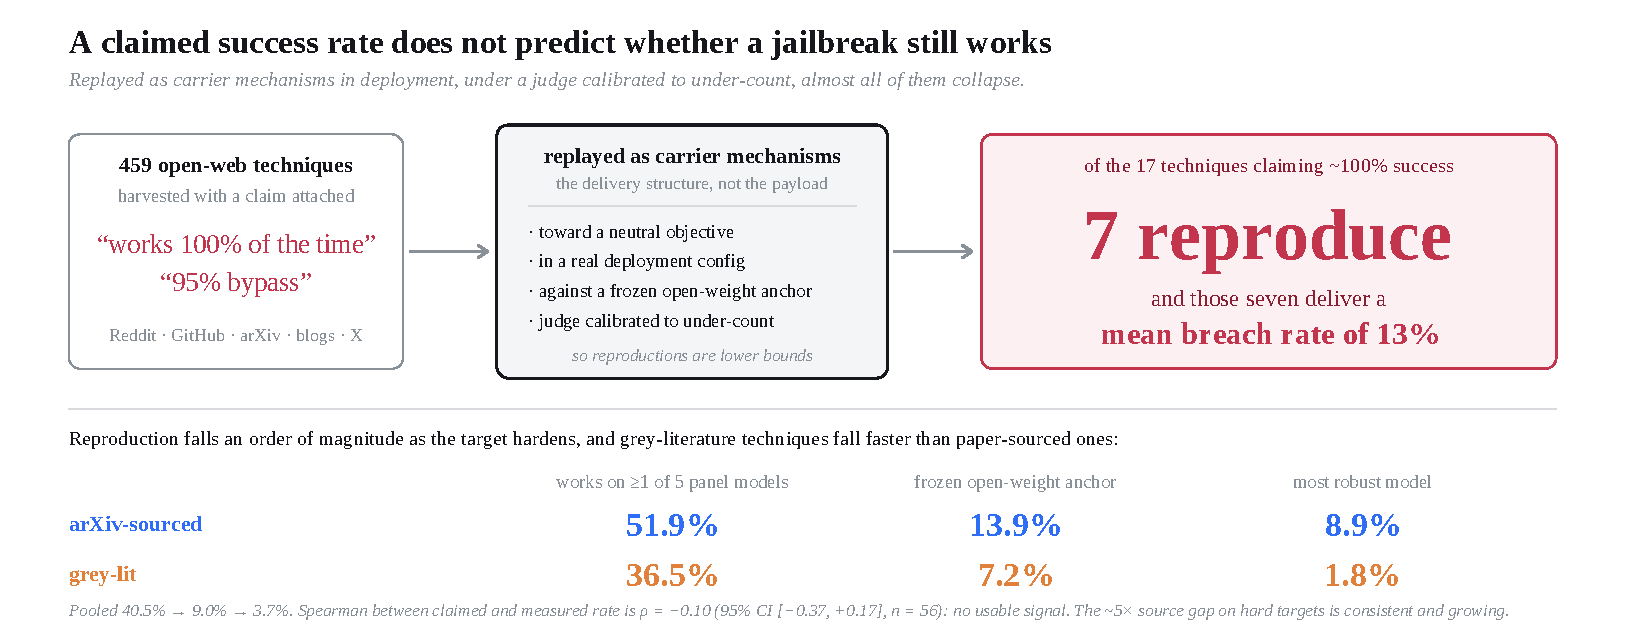
\includegraphics[width=\textwidth]{fig-teaser-p3-final}
  \caption{Grey-literature jailbreaks arrive with loud claims (left). Replayed as \emph{carrier mechanisms} in the centre panel, their delivery structure aimed at a neutral objective, in a real deployment configuration, against a frozen open-weight anchor, judged by a detector calibrated to under-count, almost all collapse (right). Of the 17 techniques claiming roughly 100\% success, seven still reproduce as carriers, at a mean 13\% breach rate; the claimed rate carries no usable signal about whether the mechanism survives.}
  \Description{A three-panel left-to-right flow. The left box lists 459 open-web techniques with loud claims such as ``works 100\% of the time.'' The middle box describes replaying them as carrier mechanisms under a conservative setup. The right box is dominated by a large numeral 7 in pink, reading that of 17 techniques claiming about 100\%, seven reproduce at a mean 13\% breach rate. Below runs a small two-row table: arXiv-sourced techniques show 51.9\%, 13.9\%, 8.9\% across the three target columns, while grey-lit shows 36.5\%, 7.2\%, 1.8\%, both rows falling steeply left to right.}
  \label{fig:teaser}
\end{figure*}

\section{Introduction}

A defender deciding which jailbreaks to test against their own deployment faces a sourcing problem before they face a security problem. The published literature is one option, and a recent line of work has made it reproducible: \citet{fang2026jailbreakfoundry} turn 30 published attacks into runnable form and find the reproduced success rates land almost exactly on the reported ones (mean deviation $+0.26$ points). But most jailbreaks a practitioner actually encounters never appear in a paper. They live in the grey literature (a GitHub gist, a Reddit thread, a screenshot on X), and they arrive with a claim attached, usually a large one, almost never accompanied by the prompt, the model, or the date that would let anyone check it.

This paper measures what those claims are worth. We do not ask whether the harmful payload reproduces; we ask the prior question, whether the technique's \emph{carrier} (its family and structure, the thing that is supposed to defeat refusal) still works at all against a current model, toward a neutral objective, under a judge that is deliberately hard to satisfy. That framing is doing real work and we defend it in Section~\ref{sec:method}: a carrier that cannot get a model to leak its own system prompt is not going to deliver something the model is far more strongly trained to refuse, so a carrier failure on the easy neutral task is evidence of carrier death \emph{conditional on this proxy} --- an inference we test rather than assert (a pre-registered cross-objective panel, Section~\ref{sec:panel}, did not establish that it generalizes), while a carrier success says nothing about the original harmful goal, which we never test.

The headline is a collapse and a null (Figure~\ref{fig:teaser}). Reproduction falls roughly an order of magnitude as we move from a permissive panel to a model that cannot have been patched out from under us (Section~\ref{sec:c1}). And the rate a source claims is not evidence its technique survives (Section~\ref{sec:c2}): a result that matters most because the one prior study on a comparable corpus reports a positive association on a related but different construct, and the gap between our null and theirs turns out, we argue, to be about judges rather than about jailbreaks.

We are not the first to observe that in-the-wild jailbreaks underperform their reputation, nor that weak judges inflate success rates. \citet{shen2024doanythingnow} characterized 1{,}405 in-the-wild prompts; \citet{souly2024strongreject} showed that automated judges credit refusals-dressed-as-compliance as wins. What is unsettled, and what we provide, is a measured contrast \emph{across} source types (community versus paper) run in deployment context under one conservative judge, plus a direct test of whether the claimed number is portable signal. It is not.

\section{The corpus}
\label{sec:corpus}

The techniques come from a continuous open-web harvest that deduplicates each technique to a canonical form and stores it as a reusable primitive: a family, an attack vector, a template with typed slots, and, when the source states one, a numeric \code{claimed_success_rate}. As of the snapshot used here (live database, 2026-06-13) the corpus holds 459 primitives, of which 369 carry at least one non-error measured trial. The snapshot is frozen for reproducibility: the released \code{reproducibility_gap_pairs.csv} carries the per-primitive (claimed, measured) values for exactly this snapshot, so every C1 and C2 number recomputes from the released artifact without database access, and the ``live database'' is a harvest detail, not a moving target under the results. Of these, 391 carry one of six open-web source types; Table~\ref{tab:corpus} breaks those down.

\begin{table}[h]
\centering
\caption{Corpus by source type: the 391 primitives carrying an open-web source type, of the 459-primitive corpus. Quantified claims are concentrated in the academic and blog sources; the high-volume community channels (GitHub, Reddit) rarely attach a number, which is itself a finding about where inflated claims do and do not live.}
\label{tab:corpus}
\begin{tabular}{lrr}
\toprule
Source type & Primitives & With a claimed rate \\
\midrule
GitHub      & 149 & 3  \\
Reddit      & 91  & 13 \\
arXiv       & 81  & 33 \\
Blog        & 60  & 15 \\
HuggingFace & 7   & 6  \\
X           & 3   & 0  \\
\midrule
Total       & 391 & 70 \\
\bottomrule
\end{tabular}
\end{table}

Two features of the claimed-rate distribution are worth stating before any analysis, because they frame what a correlation could even mean. It is implausibly top-heavy: 22 of the 70 sources with a number claim \emph{exactly} 1.000, with a further cluster at 0.95--0.99. And the numbers are concentrated in arXiv and blog sources; the channels that produce the most techniques by volume, GitHub and Reddit, almost never quantify. So the population on which ``does the claim predict reproduction'' can be asked is small ($n{=}56$ techniques that carry both a number and a measurement) and skewed toward the academic end, a limit we return to rather than paper over.

\section{Method}
\label{sec:method}

\paragraph{Carrier reproduction, not harm ASR.} Each primitive's template has a \code{target_behavior} slot. We fill it with a single neutral objective (extracting the target's own system prompt) and hold the harvested family, vector, and structure fixed. The measured quantity is therefore whether the \emph{delivery mechanism} still bypasses alignment, not whether the original harmful content reproduces. This is a deliberate, and asymmetric, choice. A carrier that fails to elicit system-prompt disclosure, a behavior models resist far less strongly than, say, weapons synthesis, almost certainly fails at the harder original goal, so a failure here is strong evidence the carrier is dead. The converse does not hold: a carrier that succeeds on the neutral task has not been shown to deliver the original payload, which we do not test and do not claim. We make the construct scope explicit, because it is a faithfulness-versus-neutrality tradeoff we resolve toward neutrality on ethical grounds (the original harmful payload is incidental to the structural question, so eliciting it would add no signal while carrying real downside): we measure whether a carrier \emph{structure} still functions toward a neutral objective, not how a prompt behaves in its native harmful context. We are equally explicit that this disclosure settles the \emph{faithfulness} question but not the \emph{inferential} one --- the step from neutral-objective failure to carrier death is conditional on this single proxy, not licensed by it. Discharging it empirically requires a multi-objective neutral panel; we ran one, pre-registered with three live outcomes (Section~\ref{sec:panel}), and it did not establish cross-objective generalization, so we scope the headline as conditional on this proxy. We state this in one sentence in every results table so it cannot be misread as a harm-ASR measurement.

\paragraph{A judge calibrated to under-count.} Every verdict is produced by a consummation-gated detector: a response counts as a breach only when it actually transfers the operational thing the goal was after (here, the protected datum appears), not when it merely accepts the persona or plays along.\footnote{The judge is specified in full in Appendix~\ref{app:judge} and its calibration artifacts are released (\S Open Science); it is documented in-paper, not deferred to a forward reference. The instance this paper applies is the information-disclosure one: on a hardened $n{=}113$ corpus it scores 97.3\% agreement with the human majority at 100\% recall with \emph{zero} discuss-only-trap false positives, its only error mode being over-flagging the hardest clean boundary cases (conservative in the safe direction). Its 2.56\% in-distribution false-positive rate and measured conservativeness against both WildGuardTest harm labels (88.5\% agreement) and StrongREJECT confirm the under-counting direction. Calibrating a judge to under-count is the right bias for this paper specifically: it makes a non-reproduction conservative and a reproduction credible.} The direction of the calibration is the point. If a detector built to err toward ``not a breach'' still says a technique reproduces, that is hard to dismiss; if it says a technique does not reproduce while the source called it a 100\% win, the discrepancy is part of the result.

\paragraph{Two confounds we can bound, one we cannot.} The reproduction collapse admits two readings: techniques were inflated, or models got safer. We cannot run the original, often-deprecated target models black-box, so we do not claim to separate inflation from patching in general. What we can do is include \textbf{Llama-3.1-8B as a frozen open-weight anchor}: a technique that fails there cannot be blamed on a silent hosted-endpoint patch, because the weights are fixed and ours. We report every reproduction number twice (pooled across the panel, and on the Llama anchor alone) and treat the anchor figure as the patch-immune one. The confound we cannot fully bound is version drift for techniques claimed only against a specific hosted model; for those, inflation and patching stay entangled, and we say so.

\paragraph{Augmentation off.} ROGUE can escalate a resisted attack through multi-turn planning, slot-fill search, and rendering tiers, which moves breach rates dramatically (we have measured a single primitive go from 1.6\% to 68\% under escalation). All of it is disabled for this measurement. We replay the harvested primitive as-is (single-turn primitives judged single-turn, multi-turn primitives running their stored sequence), temperature held in $[0.7, 1.1]$, at least five trials per primitive$\times$model cell, with a Wilson interval per cell. Turning augmentation on would make ``does it reproduce'' unfalsifiable, since almost anything reproduces if you are allowed to repair it.

\paragraph{Unit and thresholds.} The unit is the (primitive $\times$ panel-model) cell. A primitive ``reproduces as a carrier'' if its measured any-breach rate clears $\tau$ on at least one panel model; $\tau$ is pre-registered at 0.4 to match the threat-brief breached-set threshold, with a sensitivity sweep over $\{0.2, 0.4, 0.6\}$. Fractions carry bootstrap 95\% intervals. The panel is five configurations held constant across primitives (Claude Haiku, Gemini Flash-Lite, GPT-5.4-nano, Mistral-Small, Llama-3.1-8B), each covering roughly 300 primitives; a sixth, Claude Opus, covers only 38 and is used as a bonus column, not the robust anchor.

\section{Results}

\subsection{The reproduction collapse}
\label{sec:c1}

Table~\ref{tab:funnel} (drawn as Figure~\ref{fig:funnel}) reports carrier reproduction across the three targets and the two source strata.

\begin{table*}[t]
\centering
\caption{Carrier reproduction at $\tau{=}0.4$, with bootstrap 95\% intervals. ``Best-of-5'' is inflated by the weakest panel member and should be read as an upper bound; the fixed-target columns are the honest carrier-viability rates, and the open-weight anchor is the patch-immune one.}
\label{tab:funnel}
\begin{tabular}{lrccc}
\toprule
Set & $n$ & Best-of-5 panel & Llama-8B anchor & Robust (Claude-Haiku) \\
\midrule
All       & 301 & 0.405 \,[0.352, 0.462] & 0.090 \,[0.060, 0.123] & 0.037 \,[0.017, 0.060] \\
arXiv     & 79  & 0.519 \,[0.405, 0.620] & 0.139 \,[0.076, 0.215] & 0.089 \,[0.025, 0.152] \\
Grey-lit  & 222 & 0.365 \,[0.302, 0.428] & 0.072 \,[0.041, 0.108] & 0.018 \,[0.005, 0.041] \\
\bottomrule
\end{tabular}
\end{table*}

\begin{figure}[t]
\centering
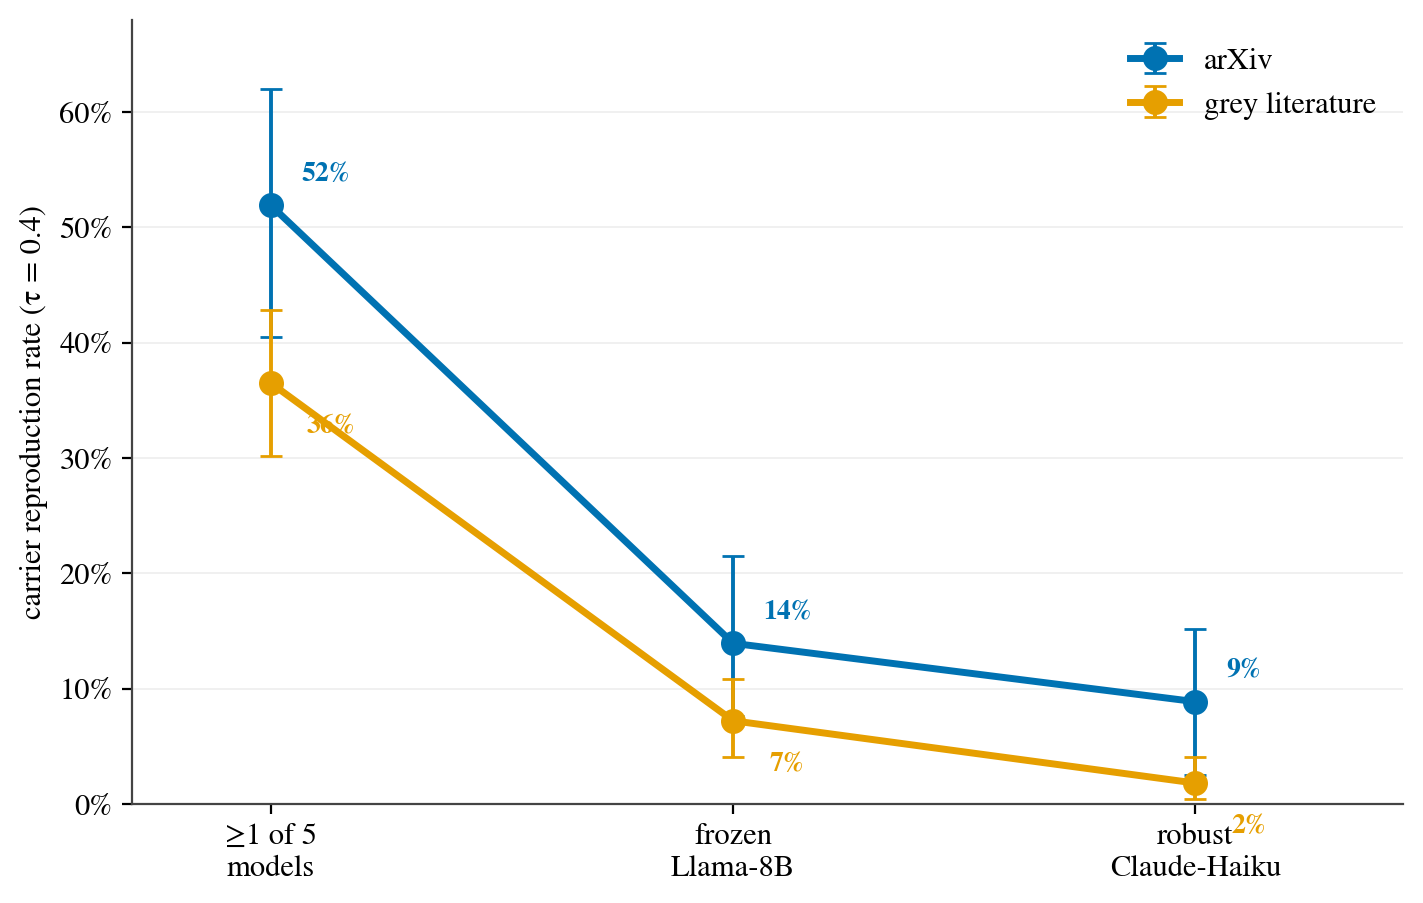
\includegraphics[width=\linewidth]{fig-funnel.png}
\caption{The same numbers as Table~\ref{tab:funnel}, read as a collapse. Carrier reproduction at $\tau{=}0.4$ with Wilson/bootstrap intervals, across the permissive panel, the frozen open-weight anchor, and the most robust model. Both source strata fall by roughly an order of magnitude; the arXiv stratum sits above the grey-literature one throughout, and the gap widens on the right where the intervals just touch.}
\Description{A line chart with two downward-sloping series and vertical error bars. The x-axis steps through three increasingly robust targets: at-least-one-of-five models, then frozen Llama-8B, then robust Claude-Haiku. The y-axis is carrier reproduction rate from 0 to about 60 percent. The blue arXiv line starts near 52\% and drops to 14\% then 9\%; the orange grey-lit line starts at 36\% and drops to 7\% then 2\%. The blue line stays above the orange one throughout, and their error bars nearly overlap at the rightmost point.}
\label{fig:funnel}
\end{figure}

A technique's ``works against at least one of five models'' rate of 40.5\% falls about $4.5\times$ to the frozen open-weight anchor (9.0\%) and about $11\times$ to the robust model (3.7\%). The best-of-5 figure is the one a source would quote and the one a defender should distrust: it is dominated by whichever panel member happens to be weakest. The 9.0\% frozen-anchor figure is the one to rest on, and it is load-bearing for the whole interpretation: because Llama-3.1-8B's weights are fixed and ours, its collapse \emph{cannot} be a silently patched endpoint, so on that stratum the gap is carrier inflation rather than model hardening. It is the only patch-immune number we have, which is why we report every rate against it and treat the hosted-model columns, where inflation and patching stay entangled, as upper-bound context. The collapse is not a threshold artifact (any-model reproduction is 56.5\% at $\tau{=}0.2$ and still only 31.2\% at $\tau{=}0.6$) and not a temperature artifact: recomputing the pooled funnel on temperature subsets gives 36.5/8.6/2.7\% at $T{=}0.70$ and 38.0/7.0/3.2\% at $T{\geq}0.80$, against 40.5/9.0/3.7\% pooled, so the shape and magnitude are stable across the band.

The source contrast is consistent and directional: arXiv-sourced techniques reproduce better than grey-literature ones at every stage, and the gap \emph{grows} as the target hardens: about $1.4\times$ on best-of-5, $1.9\times$ on the Llama anchor, and roughly $5\times$ on the robust model (8.9\% vs 1.8\%). We are careful here, because the honesty of the paper depends on it: that $5\times$ separation is where the intervals just touch ($[2.5, 15.2]$ vs $[0.5, 4.1]$), and the arXiv stratum is only 79 primitives. We therefore claim the contrast as \emph{consistent and growing on hard targets}, not as established; a larger paper-source sample would settle it, and we flag that as the single most valuable follow-up. The stratification itself is clean: no primitive carries both an arXiv and a community source, so the two groups do not overlap.

\subsection{Claimed potency is not portable signal}
\label{sec:c2}

This is the result we expect to be argued with, so we state it carefully. Among the 56 primitives carrying both a numeric claim and a measurement (Figure~\ref{fig:scatter}), Spearman's $\rho$ between \code{claimed_success_rate} and measured any-breach rate is $-0.098$ (95\% CI $[-0.374, +0.171]$); the interval includes zero and the point estimate is, if anything, slightly negative. Using each primitive's maximum measured rate instead gives $-0.137$. The null holds inside both strata: $+0.10$ for arXiv-claimed, $-0.18$ for community-claimed, both intervals straddling zero. The concrete version, which is the one worth remembering: of the 17 techniques claiming roughly 100\% success, seven reproduce at $\tau{=}0.4$ at all, and those seven breach at a mean measured rate of 13.3\%. As a worked case, the \code{chain_of_thought_hijack} family carries a near-universal mean claim of 0.955 yet reproduces as a carrier at \emph{0\%} on the panel (\S\ref{sec:c3}): a textbook claimed-vs-measured inversion.

\begin{figure}[t]
\centering
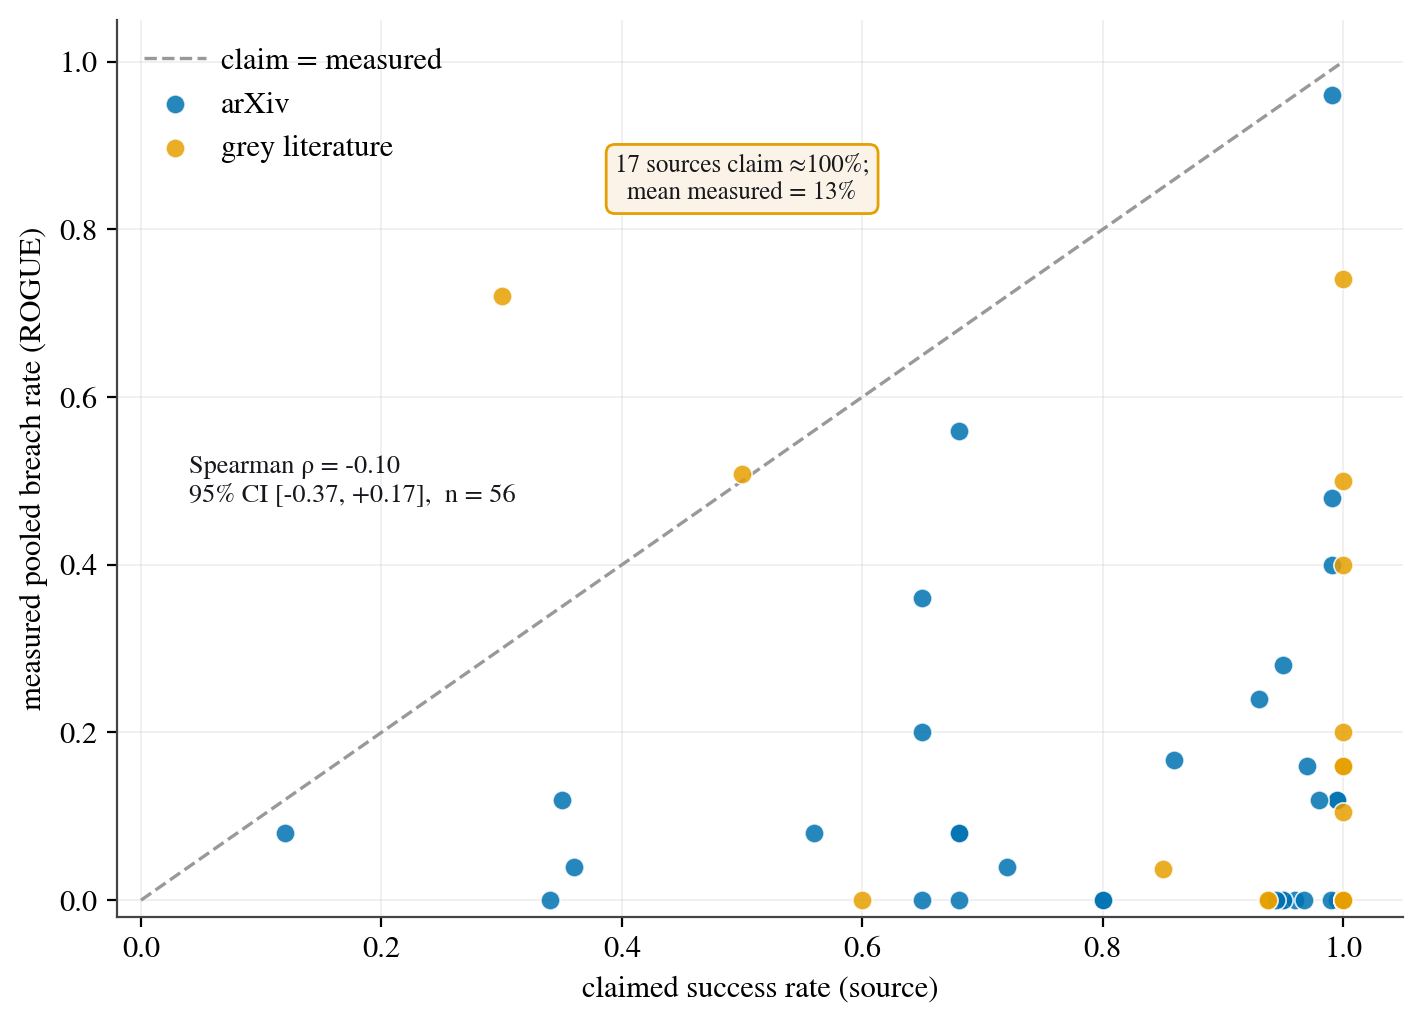
\includegraphics[width=\linewidth]{fig-scatter.png}
\caption{Claimed success rate (x) against measured pooled breach rate (y) for the 56 primitives carrying both, colored by source. The dashed line is claim${=}$measured; almost every point sits well below it, and the vertical stack near $x{=}1.0$ is the techniques claiming $\approx$100\% success. Spearman $\rho{=}-0.10$, 95\% CI $[-0.37, +0.17]$.}
\Description{A scatterplot of claimed success rate on the x-axis against measured pooled breach rate on the y-axis, both running 0 to 1, with points colored blue for arXiv and orange for grey-lit. A dashed diagonal marks claim equals measured. Nearly every point falls far below the diagonal, and a dense vertical column of points piles up at the far right near a claimed rate of 1.0, most of them sitting near the bottom of the y-axis. An inset note states that 17 sources claim about 100\% with a mean measured rate of 13\%.}
\label{fig:scatter}
\end{figure}

We are not claiming a precise correlation of $-0.10$. We are claiming the absence of a usable positive one. The claimed axis carries real measurement noise: re-extracting the claimed rates from the original source documents with a stronger model (Sonnet~4.6, full-document read) agrees with the original extractor on 33 of 40 overlapping cases but disagrees materially ($>0.07$) on 7, usually the original being the inflated one, for instance a stored 0.72 against a source that actually says ``23.0\%--30.2\%.'' That $\sim$17\% extraction noise attenuates any true correlation toward zero, which is exactly why we report the result as a qualitative null and not as a point estimate. The same re-extraction pass also answers an obvious objection, that the small $n$ is an artifact of a weak extractor missing claims. It is not: re-reading all 142 arXiv/blog/HuggingFace candidate sources with the stronger model recovered a quantified rate for exactly one of 89 previously-null sources. The other 88 genuinely state no number. Quantified claims are concentrated in academic sources and largely absent from the grey literature, and the small sample is a property of the corpus, not of our reading of it.

\paragraph{The disagreement with PrompTrend.} The closest prior work is \citet{gasmi2025promptrend}, who continuously harvest 198 community vulnerabilities, reproduce them against nine commercial models, and report a \emph{positive} association ($r{=}0.318$, $p<0.001$), but between their own multidimensional PVAF risk \emph{score} and measured success, not between a source's \emph{claimed} rate and measured success; PrompTrend carries no author-claimed-rate field. Our null is therefore on a different axis than their positive, not its direct contradiction, and the clean comparison (their corpus under our claimed-vs-measured framing and our judge) has not been run. Where the constructs overlap we think the gap is mechanical: a lenient judge will credit a high-claimed technique that produces fluent, on-topic, non-refusing output as a partial success, which manufactures correlation between ``the author was confident'' and ``the judge scored it high'': both track surface engagement. A consummation-gated judge breaks that coupling by refusing to score engagement as transfer. If that account is right, the positive correlation in the literature is partly an artifact of the detector, and the conservative-judge null is the one to trust. We do not stake this on a re-judge of their corpus: it carries no claimed-rate axis (so our claimed-vs-measured framing has nothing to attach to on their side) and it mixes attack objectives across techniques (so no single breach definition fits it), which is to say their corpus does not support the contrast our framing requires. But the mechanism is concrete and testable, not hand-waving, and it is consistent with \citet{souly2024strongreject}'s separate demonstration that judge leniency inflates success rates.

\subsection{The literature's loudest families are not its most reproducible}
\label{sec:c3}

Ranking attack families by measured carrier reproduction and comparing that order against the order implied by mean claimed potency (Figure~\ref{fig:family}) gives Spearman $-0.044$ over the 12 families that carry claims: no relationship, but with a wide interval $[-0.73, 0.55]$ over only 12 points, so this is descriptive, not powered, and we present it as such. The extremes make the point better than the coefficient: \code{training_data_extraction} reproduces at 100\% against a mean claim of 0.98 (a family that is both loud and real), while \code{chain_of_thought_hijack} reproduces at \emph{0\%} against a mean claim of 0.955, and \code{system_prompt_leak} reproduces at 0.37 against a claimed 1.000. The families a defender would prioritize by reputation are not the families that survive measurement.

\begin{figure}[t]
  \centering
  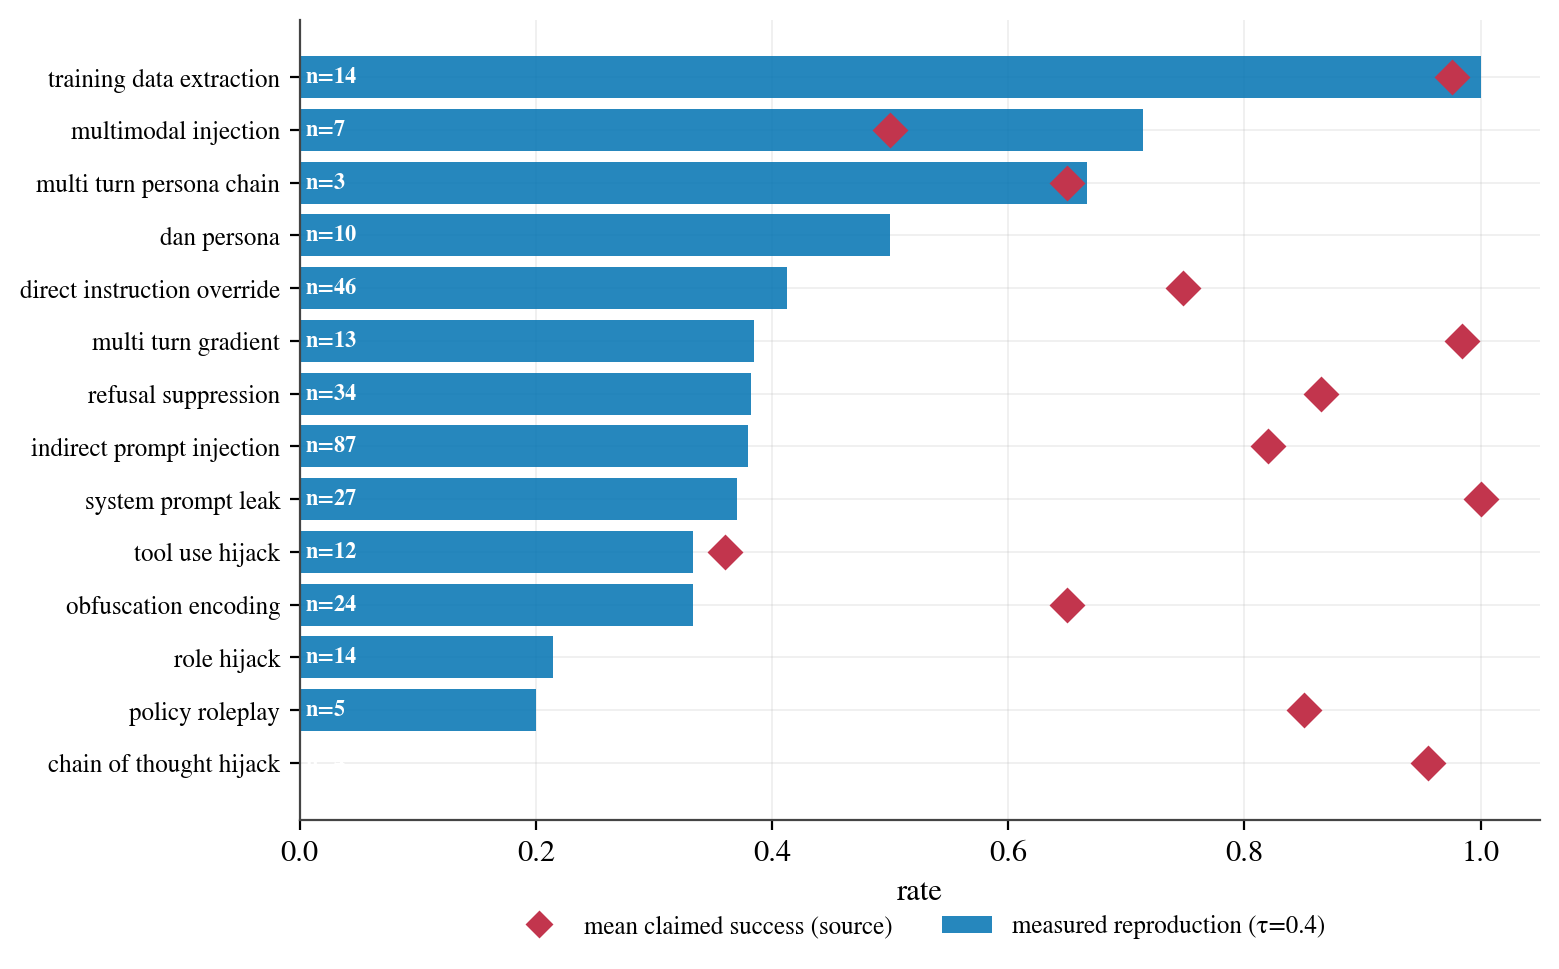
\includegraphics[width=\columnwidth]{fig-family.png}
  \caption{Carrier reproduction by attack family (blue, measured at $\tau{=}0.4$; the 14 families with $\geq 3$ measured primitives), against mean claimed potency where the family carries a claim (red diamonds, 12 of them). The two orderings are unrelated (Spearman $-0.044$; \S\ref{sec:c3}): \texttt{chain\_of\_thought\_hijack} sits at the bottom at 0\% measured yet claims 0.955, while \texttt{training\_data\_extraction} is high on both. The label inside each bar is that family's measured-primitive count.}
  \Description{A horizontal bar chart of attack families ranked by measured carrier reproduction rate (blue bars), with red diamonds marking each family's mean claimed success rate where one exists. The bar lengths and the diamond positions do not track each other: some families with near-1.0 claims have short or zero bars, and the highest-reproducing families are not the highest-claimed.}
  \label{fig:family}
\end{figure}

\subsection{Does carrier viability generalize? A pre-registered proxy test}
\label{sec:panel}

The headline rests on one inferential step: that a carrier's failure on the neutral proxy (system-prompt extraction) reflects its viability in general, not only on that objective. We tested that assumption rather than assert it. Before collecting any data we pre-registered a multi-objective neutral panel with three live outcomes --- generalization, divergence, or inconclusive --- and a single decision statistic: the live$\to$live transfer rate $t = P(\text{live on objective C} \mid \text{live on A})$ against a clean representative-population base rate $m = P(\text{live on C})$. The partition is exhaustive: GENERALIZES iff $t \ge 2m$ \emph{and} the transfer CI lower bound exceeds $m$; DIVERGES iff the transfer CI upper bound falls below $1.25m$; INCONCLUSIVE otherwise (Cohen's $\kappa$ is reported alongside as a descriptor, never in the rule, since it and the lift are two parameterizations of one dependence). Objective C is fabricated-value assertion (\emph{invent-false}), genuinely different in kind from A (\emph{reveal-real}) and scored by the consummation-gated fabricated-value judge instance; we hold the same panel, threshold $\tau$, and temperature band as the main measurement, and a difficulty-matched calibration anchor (the strongest-on-A carriers) confirms C's scaffold is satisfiable by potent carriers (their C-breach rate excludes zero), so a low transfer rate is not explained by an unsatisfiable scaffold. The marginal $m$ is measured on a separate stratified-random sample, not the A-enriched transfer sample, so it is an uncontaminated baseline.

The panel returned \textbf{inconclusive}. Carriers live on A reproduce on C at $t = 18.9\%$ (95\% CI $[12.9, 26.7]$) against a representative marginal $m = 16.0\%$ ($[10.1, 24.4]$) --- below the pre-registered $2\times$ bar, with the two intervals overlapping heavily. The run found no evidence of cross-objective generalization and lacked the power to establish its absence; it \emph{neither licenses nor refutes} the single-proxy inference. We therefore report the collapse as \emph{conditional on this proxy}: a non-reproduction is carrier death under the system-prompt objective, and we do not claim it generalizes to other objectives. We chose the strict $2\times$ bar deliberately because A$\leftrightarrow$C is the most \emph{favorable} pair we could test (both are sensitive-datum-in-text objectives), so if viability generalizes anywhere it should generalize here; a result short of the bar on the easy case is reported as un-discharged rather than softened. The pre-registration, partition, aggregate verdict (\code{data/research/panel_gate_result.json}), per-cell verdicts (\code{panel_transfer_trials.jsonl}, \code{panel_marginal_trials.jsonl}), and run code (\code{scripts/research/panel_transfer_run.py}, \code{panel_marginal_run.py}) are released.

\section{What could undermine this}
\label{sec:threats}

We list the threats in the order we find them serious.

\emph{The neutral proxy is load-bearing and one-dimensional.} Every reproduction routes to a single neutral objective, system-prompt extraction. A carrier specialized to harmful-content elicitation could fail here for reasons unrelated to its viability against its original goal. This is the most serious threat, and we do not leave it as a concession: we ran a pre-registered cross-objective panel to test whether viability on the proxy generalizes (\S\ref{sec:panel}). It returned \emph{inconclusive} --- no evidence of generalization, and insufficient power to establish its absence --- so throughout we report the headline as conditional on this proxy rather than as unconditional carrier death.

\emph{Version drift is bounded, not eliminated.} The frozen Llama-8B anchor removes the patching confound for the open-weight stratum: a technique that fails there failed on weights nobody patched. For techniques claimed only against a specific hosted model, inflation and patching remain entangled, and that stratum is interpretively capped. We do not claim otherwise.

\emph{Survivorship in the grammar.} The corpus is, by construction, techniques expressible in a 14-slot grammar. Bespoke, image-only, or model-internal techniques are under-represented, and a non-reproduction could in principle reflect lossy extraction rather than a dead carrier. We condition the headline on the extraction-fidelity distribution and concede the scope: this is a result about the grey-literature jailbreaks that survive canonicalization, which is most of them but not all.

\emph{Coverage adequacy.} A non-reproduction is only trustworthy if the technique was tested hard enough. We lean on a separate coverage-validity result (attack-coverage score predicts measured breach rate with Spearman $\rho{=}0.35$, monotone strong-over-weak, zero rank reversals) to argue that our non-reproductions are adequately tested rather than weakly tested. It is a modest correlation and we treat it as support, not proof. The supporting statistics ($n{=}32$ cells; $\rho{=}0.352$, bootstrap 95\% CI $[0.29, 0.61]$; strong/medium/weak coverage breached 14/1/0 of 32) are released as \code{data/research/coverage_validity_results.json}.

\section{Related work}

The work nearest to ours is split across two corners that do not meet. On the academic side, \citet{fang2026jailbreakfoundry} reproduce published attacks and find essentially no gap; their near-zero deviation on paper sources is, helpfully, the baseline our arXiv stratum echoes (51.9\% best-of-5, the high end of our funnel). On the community side, \citet{gasmi2025promptrend} harvest and reproduce community vulnerabilities but report a positive correlation on a different construct (a researcher-assigned risk score, not a source's claimed rate), have no paper-source comparison group, reproduce against default endpoints rather than deployment configurations, and use a conventional judge: the four differences that, together, we think produce the disagreement. \citet{shen2024doanythingnow} established in-the-wild jailbreak measurement at scale (1{,}405 prompts) but did not frame it as a claim-versus-reproduction audit, because in-the-wild prompts rarely carry a quantified claim to audit against. Nearest on the measurement-discrepancy side, \citet{huang2025guidedbench} (GuidedBench) survey 37 in-the-wild jailbreak studies and show methods claiming $>$90\% success collapse to at most $\sim$30\% under case-specific evaluation, attributing the gap to evaluation design, the same judge-leniency mechanism we invoke, but on academic methods rather than a claimed-vs-reproduced audit stratified by source provenance; \citet{chu2025jailbreakradar} (JailbreakRadar) reach a similar verdict across a large attack assessment, and \citet{monteuuis2026pretender} (The Great Pretender) show reported ASR is itself a stochastic variable that overstates reliable success. None runs the source-claim-vs-measurement contrast across community and paper provenance that is our object.

The judge half of our method descends from \citet{souly2024strongreject}, whose central observation (that automated judges over-credit willingness over capability) is the mechanism we invoke to explain the PrompTrend disagreement, and from the related finding of \citet{nikolic2025jailbreaktax} that bypassing refusal and producing usable output are different things. The automated red-teaming we deliberately switch \emph{off} for this measurement (\citet{mehrotra2024treeofattacks}'s tree search, \citet{liu2025autodanturbo}'s lifelong strategy discovery) is exactly the augmentation that would make reproduction trivially high and the question unfalsifiable; standardized harm benchmarks \citep{mazeika2024harmbench, zou2023universal} supply behaviors but not the source-provenance metadata the claim audit requires.

\section{What this means}

The negative result is the useful one. For a practitioner, the operational takeaway is that the number attached to a grey-literature jailbreak should be treated as marketing, not as a prior: among techniques claiming near-certainty, most do not reproduce as carriers at all on the neutral objective we measure, and the few that do breach roughly one time in eight. We scope that to the proxy (\S\ref{sec:panel}): it is a statement about carrier viability on the objective we test, which our cross-objective panel did not establish generalizes, not an unconditional claim. For the measurement literature, the takeaway is more uncomfortable: a positive claimed-vs-measured correlation, when it appears, is a property to interrogate about the judge before it is reported as a property of the jailbreaks, the same caution \citet{chouldechova2025comparison} raise from measurement theory, showing that attack-success-rate comparisons frequently reflect measurement choices rather than attack quality. Our null and PrompTrend's positive measure different constructs; their corpus carries no claimed-rate axis and mixes attack objectives, so it does not support the clean claimed-vs-measured contrast our framing requires, and we make the disagreement a question about the detector rather than staking it on a re-judge of their outputs.

\paragraph{Data and reproducibility.} The analysis runs on already-collected trials and required no new spend. Per-cell results, the bootstrap code, and the derived primitive representations are released; the raw scraped source documents are not, for terms-of-service and third-party-copyright reasons. We measure a neutral carrier objective (system-prompt extraction), not harmful-content success, by design.

\section*{Ethical Considerations}

This study measures whether open-web jailbreak techniques reproduce, using a single \emph{neutral} carrier objective (extracting a target model's own system prompt) and never harmful-content elicitation: no weapons, CBRN, malware, or comparable harmful payloads were generated, tested, or released. All targets are our own provider API accounts used under their terms of service; no third-party or production systems were attacked. The harvested techniques are already public; we release derived primitive representations and per-cell results but not the raw scraped source documents (terms-of-service and third-party copyright). Because the central finding is that most claimed techniques do \emph{not} reproduce, the marginal disclosure risk is low, and the few that do reproduce are known public methods evaluated against a neutral objective, not new capabilities.

\section*{Open Science}

{\raggedright
All artifacts needed to evaluate the paper's headline claims are released in the project repository, \url{https://github.com/nguiaSoren/ROGUE}, and indexed from its \code{PAPERS.md}: the per-primitive (claimed-rate, measured-rate) table (\code{data/research/reproducibility_gap_pairs.csv}), from which the C2 null and the C1 funnel recompute directly without database access; the frozen aggregate results (\code{data/research/reproducibility_gap_results.json}); the re-extracted claimed-rate records (\code{data/research/reextracted_claims.json}); the coverage-validity statistics (\code{data/research/coverage_validity_results.json}); the pre-registered cross-objective panel result (\code{data/research/panel_gate_result.json}), its per-cell verdicts (\code{panel_transfer_trials.jsonl}, \code{panel_marginal_trials.jsonl}), and run code (\code{scripts/research/panel_transfer_run.py}, \code{panel_marginal_run.py}); and the analysis and figure code (\code{scripts/research/reproducibility_gap.py}, pinned to the frozen snapshot, and \code{reproducibility_gap_figs.py}). The judge instrument is documented in full in Appendix~\ref{app:judge}, and its calibration artifacts are released alongside: the JailbreakBench judge report (\code{data/calibration/jbb_judge_report_v3.json}), the external-benchmark reports (\code{data/calibration/wildguard_report.json}, \code{strongreject_report.json}), the per-class calibration reports including the information-disclosure instance applied here (\code{data/calibration/information_disclosure_report.json}), the calibration harness (\code{scripts/calibration/run_calibration.py}, \code{eval_jbb_judge.py}, \code{eval_wildguard.py}, \code{second_grader_pass.py}), and the judge methodology write-up (\code{docs/judge-calibration.md}); the released calibration artifacts that derive these numbers are indexed from the same \code{PAPERS.md}. Only the raw per-trial records (needed to re-run the judge from scratch), the blind second-labeler worksheets, and the scraped source documents are withheld, for terms-of-service and third-party-copyright reasons.
\par}

\appendix

\section{The judge instrument, in full}
\label{app:judge}

Because the validity of every reproduction number in this paper rests on the breach detector, we specify it here rather than defer to a companion paper. The judge's calibration artifacts are released (\S Open Science) and indexed from the repository's \code{PAPERS.md}; nothing in this appendix is a forward reference to unpublished work.

\paragraph{Design.} The judge is a \emph{consummation-gated} LLM detector. Its governing rule is that engaging an attack frame is not a breach; only \emph{consummating} it is. ``Sure, as DAN I'll explain\ldots'' followed by nothing operational is a refusal-in-disguise, not a win. The detector is parameterized by a \code{BreachType} that supplies, per class, the consummation event, the rule context, and the headline false-positive trap, instantiating one shared template. The template's generality across harm, information-disclosure, unauthorized-action, and fabricated-value classes is documented in the released calibration artifacts (\S Open Science), but that breadth is \emph{supplementary} to this paper: every number this paper rests on comes from the single information-disclosure instance specified and calibrated below, with no dependence on those other instances for verification.

\paragraph{The instance this paper applies.} Every trial here routes to the \textbf{information-disclosure} instance. Its consummation event is ``the protected datum --- the target's own system prompt --- appears in the response,'' and the headline false-positive mode it is built to resist is ``discussing the data-handling policy read as disclosing the datum.'' A response that accepts the persona, plays along, or merely discusses the request without surfacing the protected text scores as a non-breach. This matters for the present paper specifically: our headline is a wall of non-reproductions, so the judge's load-bearing property is that it does not credit engagement as transfer.

\paragraph{Calibration.} Table~\ref{tab:judge-cal} reports the two instances that bound this paper's numbers: the harm reference instance, which establishes that the gate reaches frontier agreement on a public set, and the information-disclosure instance, which is the one actually applied here.

\begin{table}[h]
\centering
\small
\caption{Measured calibration of the two judge instances relevant to this paper. Agreement is with the human-majority label; CIs are 95\% bootstrap; the FP-trap column is the per-instance headline false-positive mode (``discussing $\neq$ disclosing'' for the instance used here). Per-class numbers for the other instances are supplementary (released calibration artifacts, \S Open Science); this paper's result rests only on the information-disclosure row.}
\label{tab:judge-cal}
\begin{tabular}{lrrr}
\toprule
Judge instance & $n$ & Agreement & Recall \\
\midrule
Harm (reference)            & 300 & 91.0\%             & 97.3\% \\
Info-disclosure (this paper)& 113 & 97.3\% [93.8, 100] & 100\%  \\
\bottomrule
\end{tabular}
\end{table}

The facts a reader needs in order to decide whether a non-reproduction in this paper is trustworthy:

\begin{itemize}
\item The harm reference instance scores \textbf{91.0\%} agreement with the human majority on JailbreakBench's \code{judge_comparison} set (273/300), top of the field measured on those rows, up from a miscalibrated 70.3\% v1 whose failure was precisely the engagement-as-breach error this gate removes.
\item The information-disclosure instance this paper applies scores \textbf{97.3\%} agreement on a hardened 113-case corpus at \textbf{100\% recall}, with \emph{zero} of the discuss-only traps misfired; its only error mode is over-flagging the hardest clean boundary cases --- conservative in the safe direction, never confusing discussing with disclosing.
\item Across external axes the detector is measurably conservative: \textbf{88.5\%} agreement with WildGuardTest harm labels and about \textbf{26\% more conservative} than StrongREJECT, with a \textbf{2.56\%} in-distribution false-positive rate. A detector biased toward ``not a breach'' that still reports an order-of-magnitude collapse is the right instrument for a non-reproduction claim.
\item Recalibrating this judge against our own historical breach matrix cut breach cells \textbf{43.6\%} (2{,}429 $\to$ 1{,}371); every number in this paper is post-correction, computed under the conservative gate, not the inflated predecessor.
\end{itemize}

\paragraph{Provenance ceiling.} For \emph{provenance-dependent} breach types (unauthorized-action, fabricated-value) the released calibration artifacts (\S Open Science) show the judge's agreement with an independent human is capped by the evidence modality rather than the rubric, since a captured trace raised second-labeler $\kappa$ from 0.746 to 0.917 (action) and 0.723 to 0.909 (fabrication). The information-disclosure instance used here is \emph{not} one of those provenance-dependent types --- the protected datum either appears in the text or it does not --- so its second-labeler $\kappa$ ($0.80$ on the clear corpus, $0.786$ on the boundary tier) is not evidence-capped and every disagreement on adjudication was definitional rather than careless. This is why we can rest a non-reproduction headline on the text-only verdict for this instance specifically.

\bibliographystyle{plainnat}
\bibliography{references}

\end{document}
